
\documentclass[tikz,border=5pt]{standalone}

% Core packages
\usepackage{amsmath,amssymb}
\usepackage{tikz}
\usepackage{tikz-cd}
\usepackage{pgfplots}
\usepackage{multicol}
\usepackage{xcolor}
\usepackage{caption}
\usepackage{float}
\usepackage{kotex}

% TikZ / PGF configuration
\usetikzlibrary{
  arrows.meta,
  calc,
  positioning,
  shapes.geometric,
  shapes.symbols,
  fit,
  backgrounds,
  patterns,
  matrix,
  intersections,
  decorations.pathmorphing,
  decorations.markings,
  angles,
  quotes
}
\pgfplotsset{compat=1.18}

% Reusable TikZ styles
\tikzset{
  >=stealth,
  line cap=round,
  line join=round,
  every picture/.style={line width=0.9pt},
  box/.style={draw, rounded corners, minimum width=2.8cm, minimum height=1.2cm, align=center},
  circlebox/.style={draw, circle, minimum size=1cm, align=center},
  arrow/.style={->, thick},
  dashedarrow/.style={->, thick, dashed},
  point/.style={circle, fill, inner sep=1.2pt},
  gridhelp/.style={help lines, gray!35},
  highlight/.style={fill=blue!10, draw=blue!60!black},
  3D/.style={
    x={(-0.60cm,-0.42cm)},
    y={(0.78cm,0cm)},
    z={(0cm,0.78cm)}
  }
}


\begin{document}

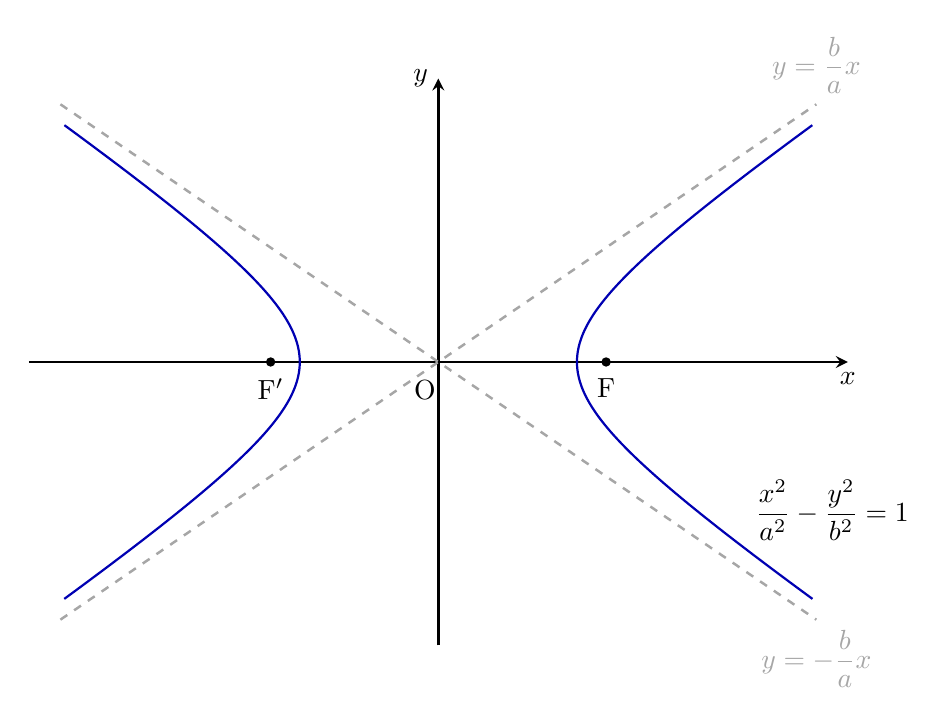
\begin{tikzpicture}[scale=0.8]
  \def\ha{2.2}
  \def\hb{1.5}
  \pgfmathsetmacro{\c}{sqrt(\ha*\ha + \hb*\hb)}
  \pgfmathsetmacro{\hSlope}{\hb/\ha}
  

  \draw[->] (-6.5,0) -- (6.5,0) node[below] {$x$};
  \draw[->] (0,-4.5) -- (0,4.5) node[left] {$y$};
  \node[below left,xshift=1mm,yshift=-1mm] at (0,0) {$\mathrm{O}$};

  \draw[blue!70!black, thick, samples=160, smooth, variable=\t, domain=-1.65:1.65]
    plot ({\ha*cosh(\t)}, {\hb*sinh(\t)});
  \draw[blue!70!black, thick, samples=160, smooth, variable=\t, domain=-1.65:1.65]
    plot ({-\ha*cosh(\t)}, {\hb*sinh(\t)});

  \draw[gray!70, dashed] (-6,-6*\hSlope) -- (6,6*\hSlope)
    node[above] {$y=\dfrac{b}{a}x$};
  \draw[gray!70, dashed] (-6,6*\hSlope) -- (6,-6*\hSlope)
    node[below] {$y=-\dfrac{b}{a}x$};
  
  \node[point,label={below:$\mathrm{F}'$}] at (-\c,0) {};
  \node[point,label={below:$\mathrm{F}$}] at (\c,0) {};

  \node[blue!70!black,text=black] at (6.25,-2.35) {$\displaystyle \frac{x^2}{a^2}-\frac{y^2}{b^2}=1$};
\end{tikzpicture}

\end{document}

